\asubsubsubsection[J. Mazzitelli]{HH production via gluon fusion at NNLO}
\label{sec:HH_NNLO}

The fusion of gluons via a heavy-quark (mainly top-quark) loop is the most important production mechanism of Higgs boson pairs at hadron colliders within the SM.
The NLO QCD corrections for this process have been known in the large-$m_t$ limit for some time \cite{Dawson:1998py}, and the NNLO cross section has also been computed within this approximation \cite{deFlorian:2013jea}.
The NLO corrections retaining the full dependence on the top-quark mass have been obtained for the first time in Refs.~\cite{Borowka:2016ehy,Borowka:2016ypz}, and have been recently confirmed by an independent calculation \cite{Baglio:2018lrj}.
On top of this, an improved NNLO prediction --labelled NNLO$_{\mathrm{FTa}}$ for full-theory approximation-- was presented in Ref.~\cite{Grazzini:2018bsd}.
This approximation is obtained by combining one-loop double-real corrections with full $m_t$ dependence with suitably reweighted real-virtual and double-virtual contributions evaluated in the large-$m_t$ limit.
Furthermore, the stability of the QCD perturbative expansion at this order has been confirmed by consistently matching the NNLO$_{\mathrm{FTa}}$ prediction with the next-to-next-to-leading logarithmic terms coming from threshold resummation \cite{deFlorian:2018tah}.

More details on the NLO results with full-$m_t$ dependence (including the effect coming from variations in the Higgs self-coupling and the contributions arising from BSM EFT operators) are provided in the following sections, therefore we focus here on the state-of-the-art NNLO prediction, i.e., the NNLO$_{\mathrm{FTa}}$ result from Ref.~\cite{Grazzini:2018bsd}.

Before focusing on the numerical results, it is worth to stress out that the NNLO cross sections presented here, as well as the NLO predictions for gluon fusion present in the following sections, are computed using the on-shell scheme for the top-quark mass renormalisation .
Some partial results on the uncertainties related to the $m_t$ scheme and scale choice have been presented in Ref.~\cite{Baglio:2018lrj} at NLO, and further studies to gauge the size of their effect on the total cross section and distributions are in progress.
This source of uncertainty is for the moment not considered in the NLO and NNLO predictions.

In Table \ref{table:HH_at_NNLO} we present results for the total cross section at $\sqrt{s} = 14$~\UTeV and 27~\UTeV.
We use the values $m_h = 125$~\UGeV for the Higgs boson mass and $m_t = 173$~\UGeV for the  on-shell top quark mass.
The NNLO PDF4LHC15 sets of parton distribution functions are used, and PDF and $\alpha_S$ uncertainties are also provided.
An estimation of the systematic uncertainty of the approximation due to missing finite-$m_t$ effects is also presented, and it is found to be at the few percent level.
For the renormalisation  and factorisation scales we use the central value $\mu_0 = M_{hh}/2$, which has been shown to provide a better convergence for the fixed order prediction \cite{deFlorian:2018tah}. We obtain the scale uncertainties via the usual 7-point scale variation.

%%====================================
{\renewcommand{\arraystretch}{1.6}
\begin{table}
\begin{center}
\begin{tabular}{|l|c|c|c|c|c|}
\hline
$\sqrt{s}$~[\UTeV] & NNLO$_{\mathrm{FTa}}$~[fb] & $m_t$ unc. & PDF unc. & $\alpha_S$ unc. & PDF$+\alpha_S$ unc. \\
 \hline
$14$ & $36.69^{+2.1\%}_{-4.9\%}$ & $\pm 2.7\%$ & $\pm 2.1\%$ & $\pm 2.1\%$ & $\pm 3.0\%$ \\
\hline
$27$ & $139.9^{+1.3\%}_{-3.9\%}$ & $\pm 3.4\%$ & $\pm 1.7\%$ & $\pm 1.8\%$ & $\pm 2.5\%$ \\
\hline
\end{tabular}
\end{center}
\caption{
Inclusive cross sections for Higgs boson pair production at NNLO$_{\mathrm{FTa}}$ for centre-of-mass energies of 14~\UTeV and 27~\UTeV. 
Scale uncertainties are reported as superscript/subscript.
The estimated uncertainty of the approximation due to finite top-quark mass effects is also presented, as well as the PDF and $\alpha_S$ uncertainties.
}
\label{table:HH_at_NNLO}
\end{table}
}
%%====================================


The NNLO$_{\mathrm{FTa}}$ predictions from Ref.~\cite{Grazzini:2018bsd} are also fully differential in the Higgs boson pair and the associated jet activity.
As an example, we present the Higgs pair invariant mass distribution at 14~\UTeV and 27~\UTeV in Figure~\ref{fig:mhh_NNLO}, together with the corresponding NLO prediction.
We can observe the strong reduction in the size of the scale uncertainties when including the NNLO$_{\mathrm{FTa}}$ corrections, and the sizeable overlap with the NLO uncertainty band (not present between the LO and NLO predictions), suggesting a significant improvement in the perturbative convergence as we move from NLO to NNLO.


%%====================================
\begin{figure}[t!]
\begin{center}
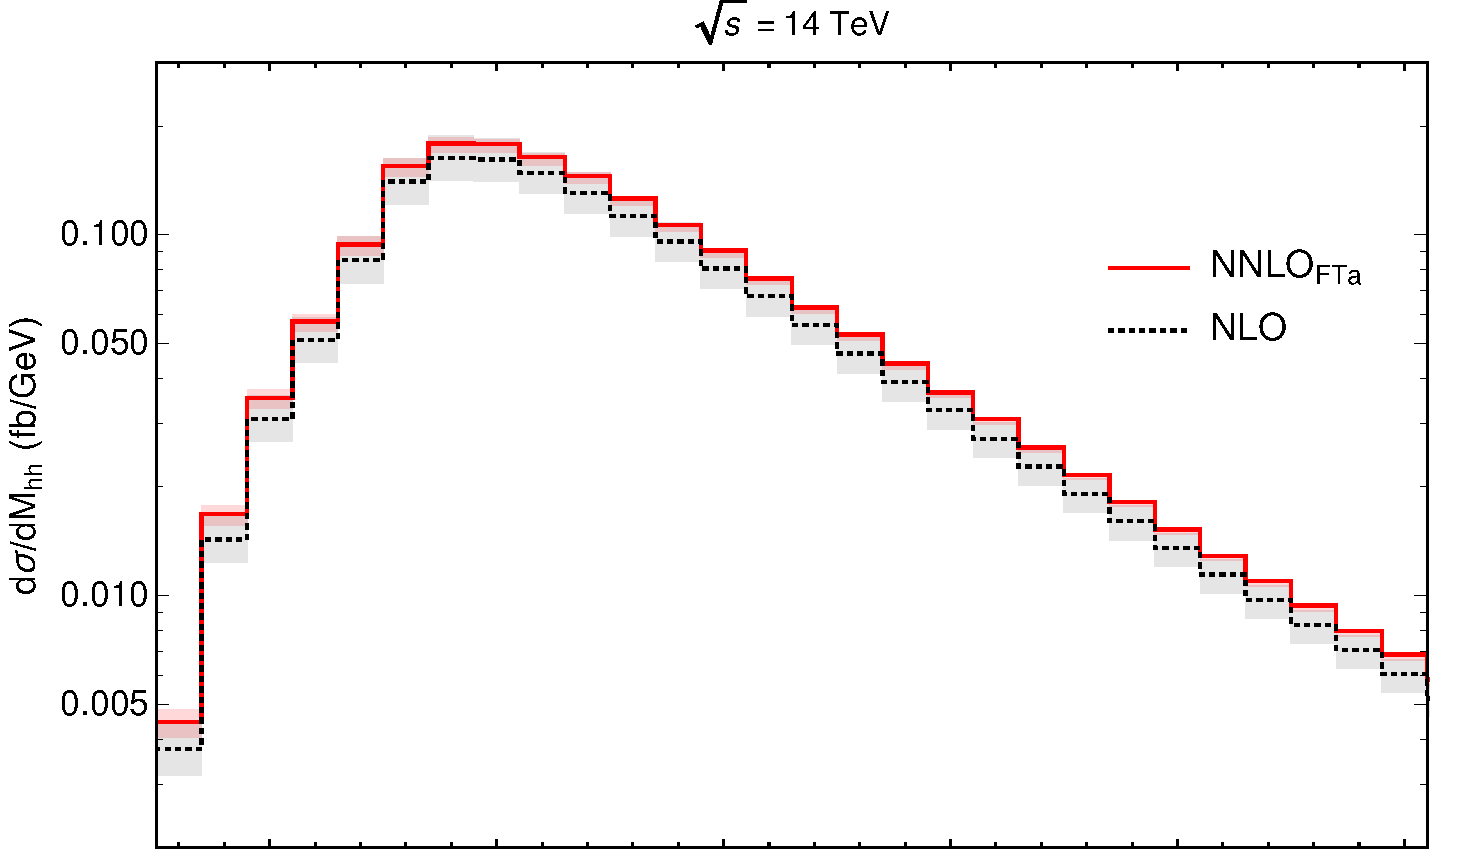
\includegraphics[width=.49\textwidth]{\main/section3/plots/14TeV_mhh}
\hfill
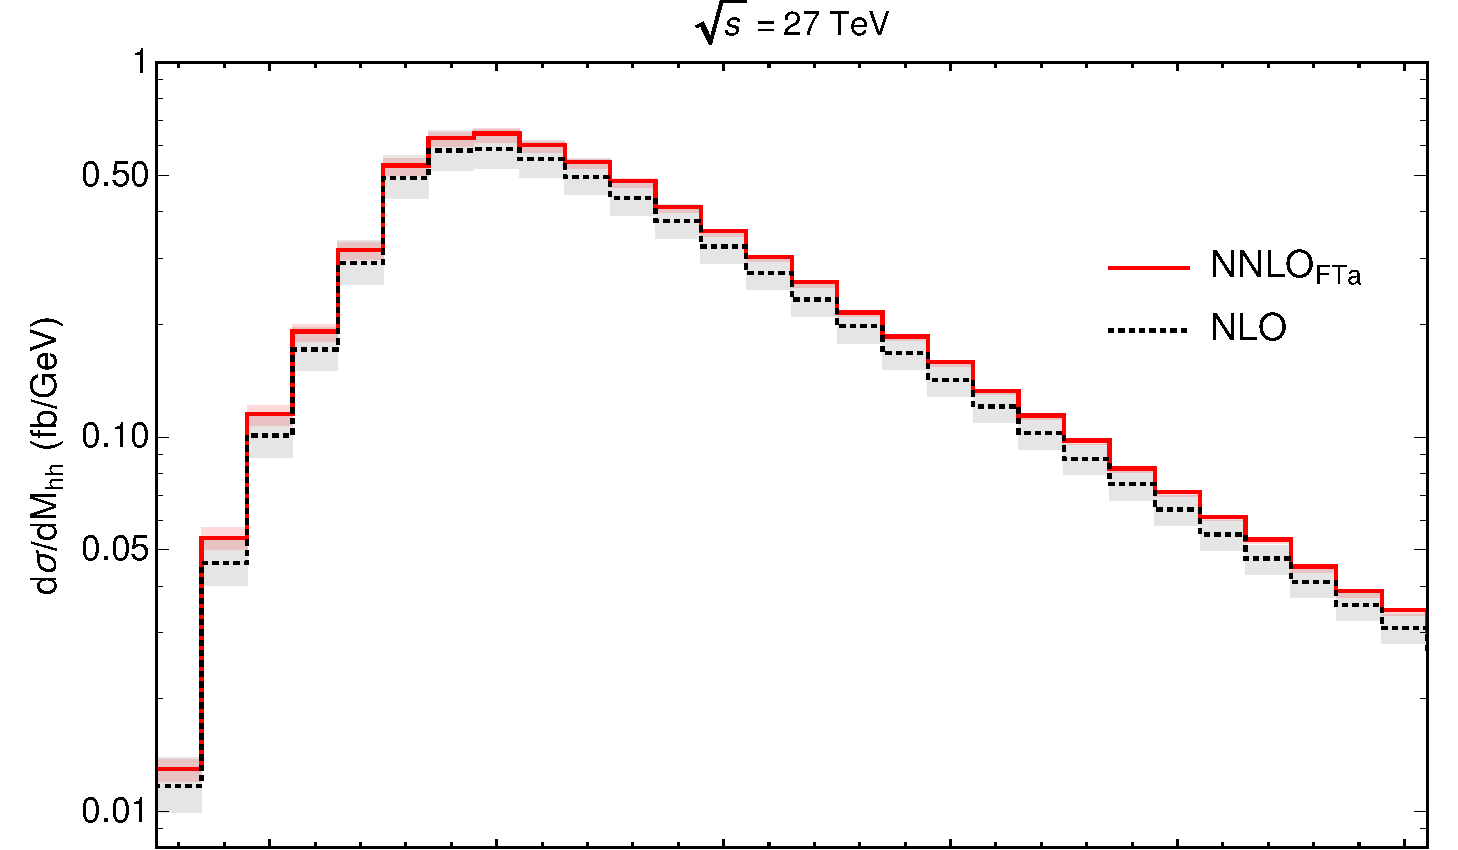
\includegraphics[width=.49\textwidth]{\main/section3/plots/27TeV_mhh}
\\
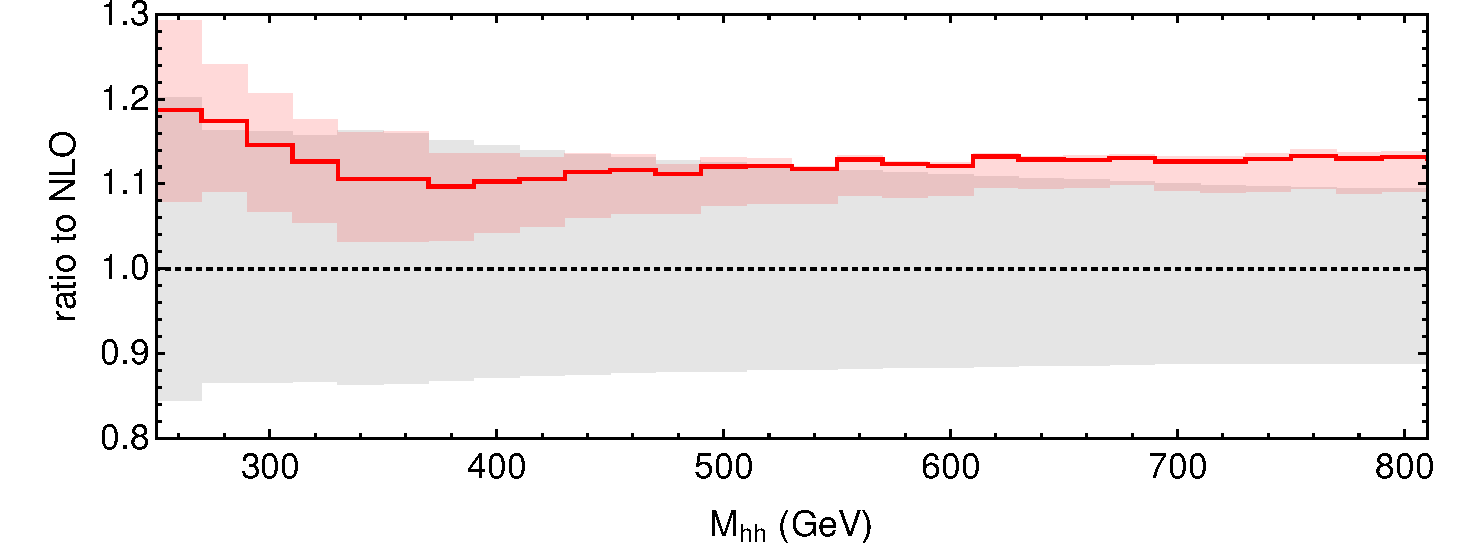
\includegraphics[width=.49\textwidth]{\main/section3/plots/14TeV_mhh_lower}
\hfill
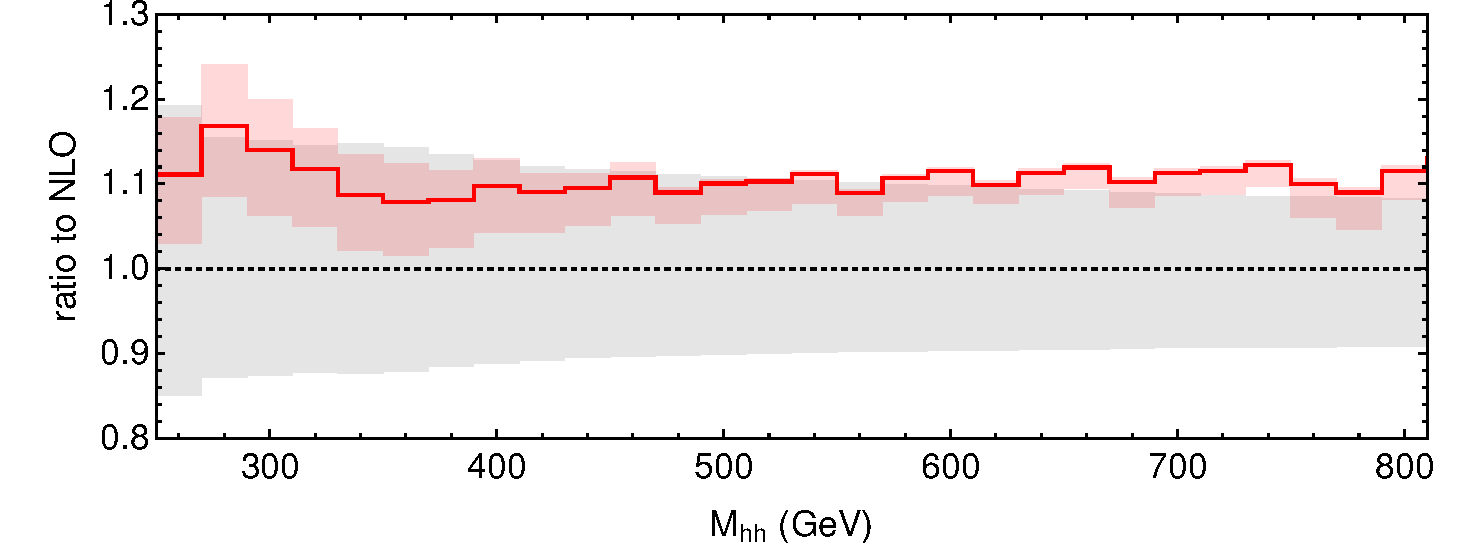
\includegraphics[width=.49\textwidth]{\main/section3/plots/27TeV_mhh_lower}
\end{center}
\vspace{-2ex}
\caption{\label{fig:mhh_NNLO}
Higgs boson pair invariant mass distribution at NNLO$_{\mathrm{FTa}}$, together with the NLO prediction, at $14\,$\UTeV (left) and $27\,$\UTeV (right). The lower panels show the ratio with respect to the NLO prediction, and the filled areas indicate the scale uncertainties.
}
\end{figure}
%%====================================
